\chapter{Arhitektura i dizajn sustava}
		

	\text Arhitektura se može podijeliti na tri podsustava:
	\begin{packed_item}
		\item Web poslužitelj
		\item Web aplikacija
		\item Baza podataka
	\end{packed_item}

	 \textit{Web preglednik} je program (Google Chrome) koji korisniku omogućuje pregled web-stranice, a ujedno je i prevoditelj. Dakle, stranica je pisana u kodu kojeg preglednik razumije te ga nakon toga interpretira kao nešto razumljivo korisniku.
	 
	 
	 \textit{Web poslužitelj} ima zadaću omogućiti komunikaciju klijenta s aplikacijom. Komunikacija se odvija preko HTTP (engl. Hyper Text Transfer Protocol) protokola. 
	 Poslužitelj je onaj koji pokreće web aplikaciju te joj prosljeđuje zahtjeve.

	 
	 \textit{Web aplikacija} obrađuje zahtjeve koje korisnik pošalje te je u komunikaciji s bazom podataka s kojom preko poslužitelja vraća korisniku odgvor u obliku HTML dokumenta vidljibog web pregledniku.
	 
	 Programski jezik korišten za izradu aplikacije je Java i Javascript. Za baze podataka korišen je pgAdmin. Aplikacija je puštena u pogon preko Heroku-a.
	 Arhitektura sustava temeljit će se na MVC (Model-View-Controller) konceptu. MVC koncept smo koristili jer je podržan u JavaSpringBoot-u kojeg koristimo te je pogodan za moguće kohezije.
	 MVC model odvaja korisničko sučelje od ostatka sustava.
	\begin{packed_item}
		\item Model sadrži razrede čiji objekti se obrađuju

		\item Pogled sadrži razrede čiji objekti služe za prikaz podataka

		\item Nadglednik (Controller) sadrži razrede koji upravljaju i rukuju korisničkom interakcijom s pogledom i modelom

	\end{packed_item}
	
		\newpage		
		\section{Baza podataka}
			
		\text U našoj web aplikaciji koristili smo relacijsku bazu podataka. Baza se sastoji od tablica koje imaju svoje atribute. Baza podataka je jako bitna da bi web aplikacija radila jer su na njoj pohranjeni svi podaci o zaposlenicima i svi skenirani dokumenti.
		\newline
		\text{Entiteti baze podataka su sljedeći:}
		\begin{packed_item}
			\item {Dokument}
			\item {Zaposlenik}
			\item {Korisnički račun}
			\item {Uloga}
			\item {Racun}
			\item {Ponuda}
			\item {Interni}
		\end{packed_item}
	
		
			\subsection{Opis tablica}
			

				
				\textbf{Zaposlenik}  Ovaj entitet sadrži osnovne informacije o zaposleniku. Sadrži sljedeće atribute: genID, PID, Name, Surname, Residence, Salary i roleID. genID je alternativni ključ dok je PID primarni ključ. Entitet je povezan s entitetom \textbf{UserAccount} preko genID i \textbf{Role} preko roleID.
				
				
				\begin{longtblr}[
					label=none,
					entry=none
					]{
						width = \textwidth,
						colspec={|X[6,l]|X[6, l]|X[20, l]|}, 
						rowhead = 1,
					} %definicija širine tablice, širine stupaca, poravnanje i broja redaka naslova tablice
					\hline \multicolumn{3}{|c|}{\textbf{Employee}}	 \\ \hline[3pt]
					\SetCell{LightGreen}genID & VARCHAR	&  kod koji zaposlenik dobije od direktora 	\\ \hline
					PID & VARCHAR	&  OIB zaposlenika 	\\ \hline
					Name	& VARCHAR &   Ime zaposlenika	\\ \hline 
					Surname & VARCHAR & Prezime zaposlenika \\ \hline
					Residence & VARCHAR &  Mjesto stanovanja \\ \hline 
					Salary & INT	& Plaća zaposlenika 		\\ \hline 
					\SetCell{LightBlue} roleID	& INT &  jedinstveni kod pozicije (uloge) 	\\ \hline 
				\end{longtblr}
				
				
				\textbf{Role}  Ovaj entitet sadržava roleID te RoleName što su ujedno i atributi. Povezan je sa entitetom \textbf{Employee} preko roleID.
				
				\begin{longtblr}[
					label=none,
					entry=none
					]{
						width = \textwidth,
						colspec={|X[6,l]|X[6, l]|X[20, l]|}, 
						rowhead = 1,
					} %definicija širine tablice, širine stupaca, poravnanje i broja redaka naslova tablice
					\hline \multicolumn{3}{|c|}{\textbf{Role}}	 \\ \hline[3pt]
					\SetCell{LightGreen}roleID & INT	& jedinstveni kod uloge 	\\ \hline
					RoleName	& VARCHAR &  ime uloge	\\ \hline 
				\end{longtblr}
			
			\textbf{Document} Ovaj entitet sadrži osnovne informacije o dokumentu. Sadrži sljedeće atribute: documentID, arhiviran, potpis te korisničko ime. Entitet je nadklasa entitetima \textbf{Receipt}, \textbf{Intern} i \textbf{Offer} te je s tim entitetima povezan preko svog documentID-a. Isto tako, povezan je s entitetom \textbf{UserAccount} preko atributa Username.
			
				\begin{longtblr}[
					label=none,
					entry=none
					]{
						width = \textwidth,
						colspec={|X[6,l]|X[6, l]|X[20, l]|}, 
						rowhead = 1,
					} %definicija širine tablice, širine stupaca, poravnanje i broja redaka naslova tablice
					\hline \multicolumn{3}{|c|}{\textbf{Document}}	 \\ \hline[3pt]
					\SetCell{LightGreen}documentID & INT	& jedinstveni kod dokumenta 	\\ \hline
					Archived	& INT &  je li dokument arhiviran (da/ne))	\\ \hline 
					Signature & INT & je li potreban direktorski potpis (da/ne) \\ \hline
					\SetCell{LightBlue} Username & VARCHAR & korisnicko ime osobe koja je skenirala dokument \\ \hline
				\end{longtblr}
			
			\textbf{Intern} Ovaj entitet je vrsta dokumenta, dakle to je specijalzacija entiteta \textbf{Document}. Sadrži atribute INT4 što je alternativni ključ, documentID što je primarni ključ i ClientName.
				\begin{longtblr}[
					label=none,
					entry=none
					]{
						width = \textwidth,
						colspec={|X[6,l]|X[6, l]|X[20, l]|}, 
						rowhead = 1,
					} %definicija širine tablice, širine stupaca, poravnanje i broja redaka naslova tablice
					\hline \multicolumn{3}{|c|}{\textbf{Intern}}	 \\ \hline[3pt]
					\SetCell{LightGreen}documentID & INT	& jedinstveni kod uloge 	\\ \hline
					INT4	& VARCHAR &  "INT" + 4 znamenke	\\ \hline
					ClientName & VARCHAR & ime klijenta \\ \hline
				\end{longtblr}		
			
			\textbf{Receipt} Ovaj entitet je vrsta dokumenta, dakle to je specijalzacija entiteta \textbf{Document}. Sadrži atribute R6 što je alternativni ključ i documentID što je primarni ključ.
				\begin{longtblr}[
					label=none,
					entry=none
					]{
						width = \textwidth,
						colspec={|X[6,l]|X[6, l]|X[20, l]|}, 
						rowhead = 1,
					} %definicija širine tablice, širine stupaca, poravnanje i broja redaka naslova tablice
					\hline \multicolumn{3}{|c|}{\textbf{Receipt}}	 \\ \hline[3pt]
					\SetCell{LightGreen}documentID & INT	& jedinstveni kod dokumenta 	\\ \hline
					R6	& VARCHAR &  "R" + 6 znamenki	\\ \hline
				\end{longtblr}	
			
			\textbf{Offer}	Ovaj entitet je vrsta dokumenta, dakle to je specijalzacija entiteta \textbf{Document}. Sadrži atribute P9 što je alternativni ključ te documentID što je primarni ključ.	
				\begin{longtblr}[
					label=none,
					entry=none
					]{
						width = \textwidth,
						colspec={|X[6,l]|X[6, l]|X[20, l]|}, 
						rowhead = 1,
					} %definicija širine tablice, širine stupaca, poravnanje i broja redaka naslova tablice
					\hline \multicolumn{3}{|c|}{\textbf{Offer}}	 \\ \hline[3pt]
					\SetCell{LightGreen}documentID & INT	& jedinstveni kod uloge 	\\ \hline
					P9	& VARCHAR &  "P" + 9 znamenki	\\ \hline
				\end{longtblr}
			
			\textbf{UserAccount} Ovaj entitet sadrži podatke o korisnčkim računima. Sadrži sljedeće atribute: Username što je ujedno i primarni key, password, email, enabled i PID što je strani ključ. Entitet je povezan s entitetom \textbf{Document} preko atributa Username i s entitetom \textbf{Employee} preko atributa PID.
				
				\begin{longtblr}[
					label=none,
					entry=none
					]{
						width = \textwidth,
						colspec={|X[6,l]|X[6, l]|X[20, l]|}, 
						rowhead = 1,
					} %definicija širine tablice, širine stupaca, poravnanje i broja redaka naslova tablice
					\hline \multicolumn{3}{|c|}{\textbf{UserAccount}}	 \\ \hline[3pt]
					\SetCell{LightGreen}Username & VARCHAR	& korisničko ime	\\ \hline
					password	& VARCHAR &  šifra	\\ \hline 
					email & VARCHAR & mail adresa \\ \hline
					\SetCell{LightBlue} PID & VARCHAR & oib zaposlenika \\ \hline
				\end{longtblr}
				
			
			
			
			
			
			
			
			
			
				
			
			\subsection{Dijagram baze podataka}
				
				\begin{figure}[H]
					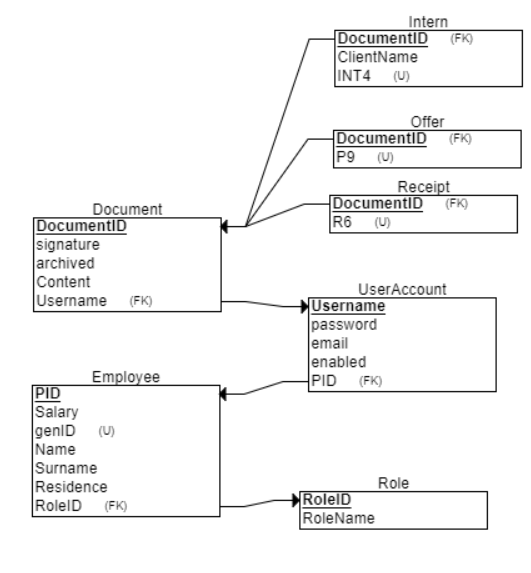
\includegraphics[scale=0.58]{slike/REL_schema.png} %veličina slike u odnosu na originalnu datoteku i pozicija slike
					\centering
					\caption{Relacijski model baze podataka}
					\label{REL}
				\end{figure}
				
				
			
		
			
			
		\section{Dijagram razreda}
		
			
			\begin{figure}[H]
				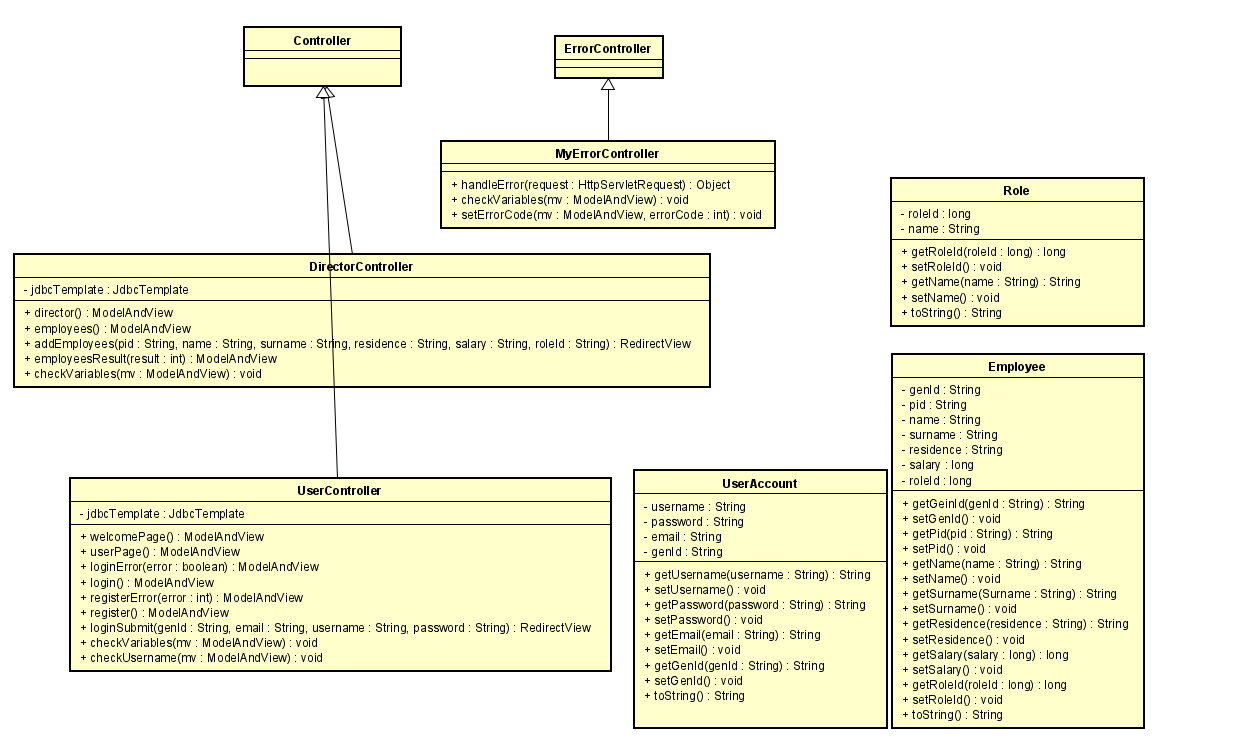
\includegraphics[scale=0.58]{slike/DijagramRazredaAlfa.png} %veličina slike u odnosu na originalnu datoteku i pozicija slike
				\centering
				\caption{Dijagram razreda}
				\label{DR1}
			\end{figure}
		
		
		
			
			\textbf{\textit{dio 2. revizije}}\\			
			
			\textit{Prilikom druge predaje projekta dijagram razreda i opisi moraju odgovarati stvarnom stanju implementacije}
			
			
			
			\eject
		
		\section{Dijagram stanja}
			
			Dijagram stanja prikazuje prijelaze iz jednog stanja u drugo na temelju različitih događaja. U prvom planu je zaposlenik koji ima mogućnost odjaviti se sa profila, deaktivirati profil, vidjeti popis svih dokumenata koje je skenirao te upload dokumenata. Ukoliko uploada dokumente, mora ih skenirati pomoću OCR-a. Nakon toga dobiva listu skenova te gleda kako su skenovi ispali. Dokumenti kod kojih je OCR uspješno izveden šalju se revizoru na daljnju obradu, a ukoliko OCR nije uspješan dokument se ne šalje nego se preskoči.
			
			\begin{figure}[H]
				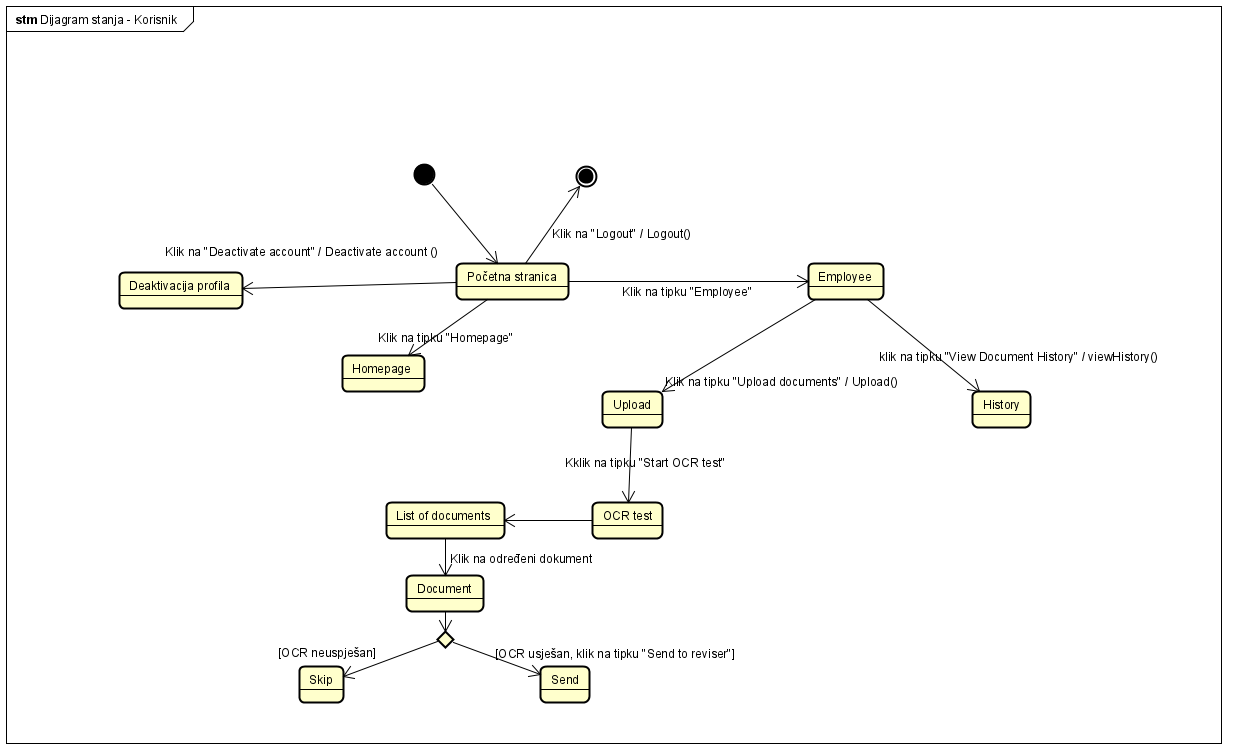
\includegraphics[scale=0.5]{slike/Dijagram stanja.png} %veličina slike u odnosu na originalnu datoteku i pozicija slike
				\centering
				\caption{Dijagram stanja}
				\label{DS}
			\end{figure}
			
			\eject 
		
		\section{Dijagram aktivnosti}
			
			 Dijagram aktivnosti odnosi se na korisnika, njegovo uploadanje dokumenata, skeniranje dokumenata i slanje dalje drugim zaposlenicima. Dakle, korisnik se prvo mora prijaviti u sustav. U bazi se provjeravaju podaci i ako je sve točno, prijava je uspješna. Ukoliko korisnik nije u bazi podataka, ima priliku opet se prijaviti. Nakon što se korisnik prijavio ima mogućnost da skenira dokument. Web aplikacija provede OCR, skenirani dokument se spremi u bazu podataka. Korisnik vidi kako izgledaju skenirani dokumenti te bira one koji su dobri. Ukoliko se radi o zaposleniku, on šalje skenirane dokumente revizoru. Revizor dokument prosljeđuje računovođi koji prosljeđuje direktoru na potpis. Korisnik ima obavijest kada mu netko pošalje dokument. Na kraju se dokument arhivira čime je proces završen.
			 
			 \begin{figure}[H]
			 	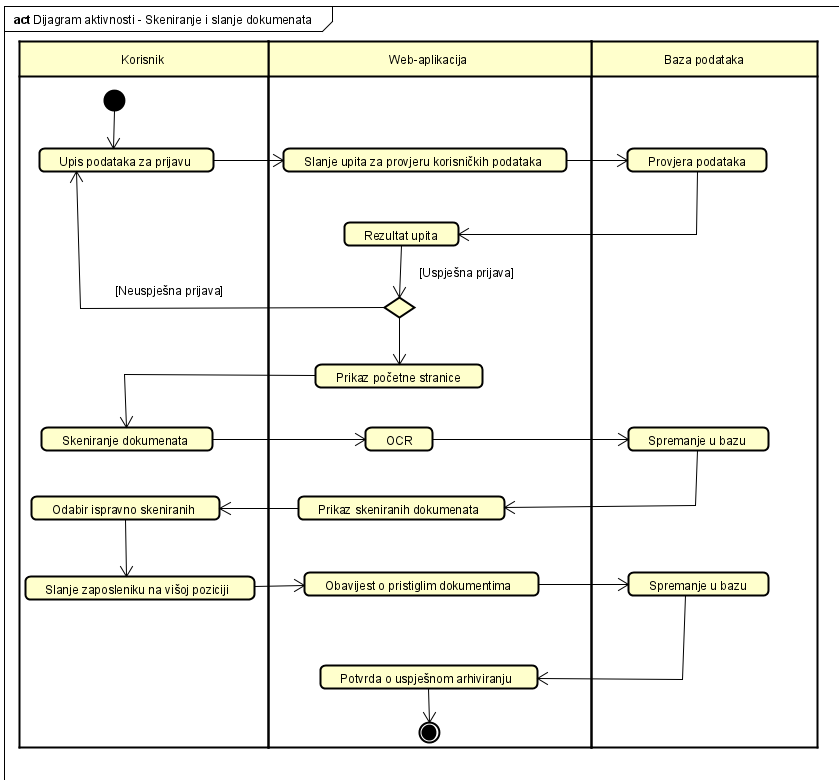
\includegraphics[scale=0.5]{slike/Dijagram aktivnosti.png} %veličina slike u odnosu na originalnu datoteku i pozicija slike
			 	\centering
			 	\caption{Dijagram aktivnosti}
			 	\label{DA}
			 \end{figure}
			 
			
			\eject
		\section{Dijagram komponenti}
		
			 Dijagram komponenti prikazuje organizaciju i međuovisnost komponenti te internu strukturu aplikacije. Frontend je pisan u HTML-u i CSS-u te je on povezan s aplikacijom. Baza podataka također komunicira sa aplikacijom te se iz nje uzimaju potrebni podaci pomoću SQL upita. ConditionChecker za svaku ulogu provjerava o kome se radi. Rest poslužuje aplikaciju te povezuje frontend s backendom. Uz to, komunicira s Controllers koji je dio MVC strukture. Potrebni podaci se šalju u bazu podataka, a za to je zaslužan "dao". Baza podataka se tako cijelo vrijeme ažurira prilikom ukoliko se nešto mijenja za vrijeme rada aplikacije.
			 
			 
			  \begin{figure}[H]
			 	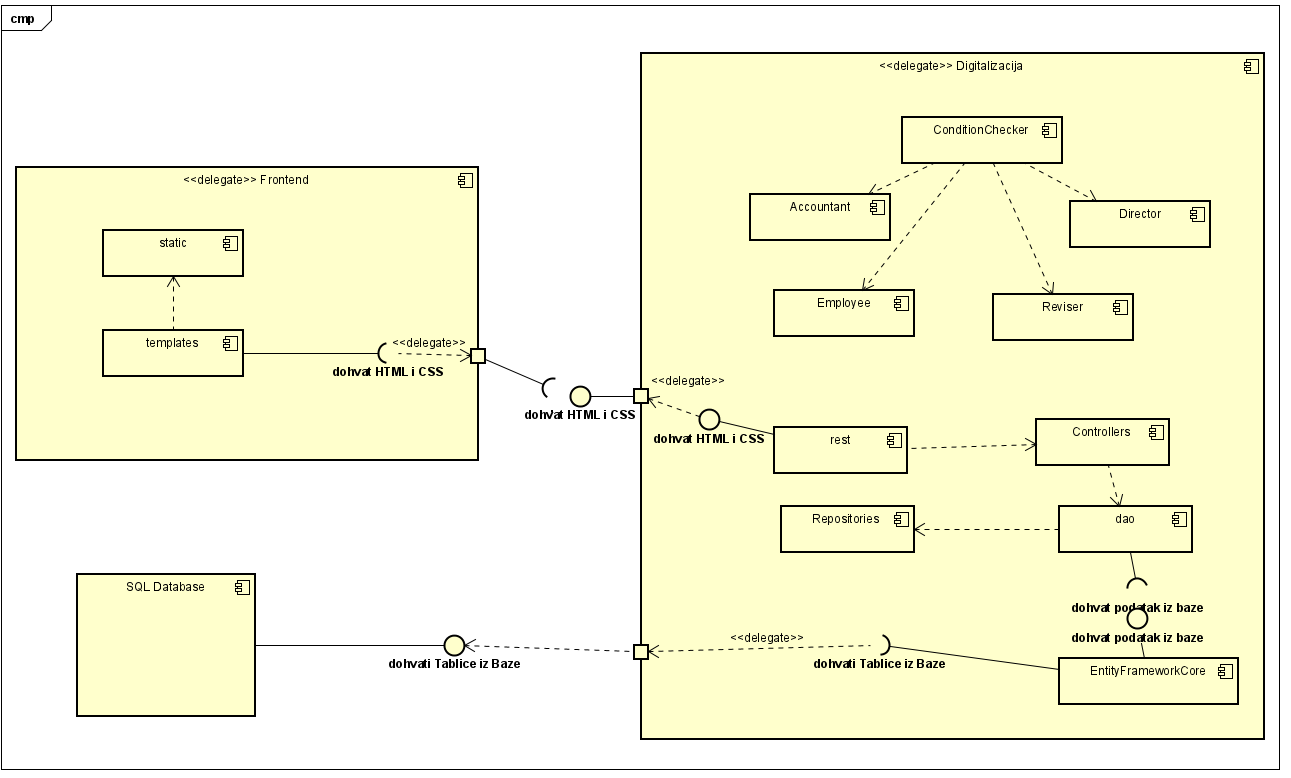
\includegraphics[scale=0.5]{slike/Dijagram komponenti.png} %veličina slike u odnosu na originalnu datoteku i pozicija slike
			 	\centering
			 	\caption{Dijagram komponenti}
			 	\label{DK}
			 \end{figure}
			 